\documentclass[a4paper]{article}

\usepackage{fullpage} % Package to use full page
\usepackage{parskip} % Package to tweak paragraph skipping
\usepackage{tikz} % Package for drawing
\usepackage{url}
\usepackage{amsmath}
\usepackage{hyperref}
\usepackage{multirow}
\usepackage{tabularx}


\title{Image Processing Library}
\author{Navneel Mandal \& Mayank Singh Kushwaha}
\date{Feb 17th, 2019}

\begin{document}

\maketitle

\section{Introduction}

It is the first Assignment of the COP290 course. The whole Assignment is sub divided into 3 sub-tasks, each of which have different objectives. The first sub-task aims at creating some functions to use for the second and the third sub-task. The second sub-task aims at using different libraries for doing matrix multiplication, while the third sub-task implements the LeNet Architecture to identify handwritten digits from the MNIST database.

\section{Creating Functions for later use}

For the first sub-task we create many functions which are to be used later in the subsequent sub tasks. The table below shows the function and the arguments it takes when running.

\subsection{Running this sub-task}
To run this sub-task independently, we first compile the necessary files by running the command
\begin{verbatim}
    make main
\end{verbatim}
Once compiled, we get our .out file as main.out,which can be used to execute the functions with correct parameters. A list of all the commands has been provided in Table \ref{tab:title}. 

A very detailed description of each of the functions in provided in the README.md. It is encouraged to go through that file.

\subsection{Output}
The default output comes in the terminal itself but the display may be illegible for bigger size matrix. Therefore there is a Output.txt file, where every output of the main.out file is stored.

\section{Comparing Matrix Multiplication}
This is the second sub-task, where we use different libraries to compare the speeds of various libraries for matrix multiplication. We compare 3 libraries:
\begin{enumerate}
\item Pthreads implementation of Matrix Multiplication
\item OpenBlas Implementation
\item Intel MKL Implementation
\end{enumerate}
\subsection{Installation}
\subsubsection{Pthreads}
Pthreads comes installed in UNIX systems, so there is no need for further installation. We, for this assignment, settled on 5 as the number of threads after running for various values and seeing that this one gave the lowest time for the majority of the sizes we tested for. For compilation purposes, though the command 
\begin{verbatim} <your_command> -lpthreads \end{verbatim}
must be used. Although in this case, just running
\begin{verbatim}
    make plot_pthreads
\end{verbatim}
will suffice.
\subsubsection{openBlas}
To install openBlas, one can directly execute the shell script provided
\begin{verbatim}
    ./install_openblas.sh
\end{verbatim}
For compilation, similarly
\begin{verbatim} <your_command> -lopenblas \end{verbatim}
must be used. Although in this case, just running
\begin{verbatim}
    make plot_openblas
\end{verbatim}
will suffice.
\subsubsection{MKL}
To install MKL, run the script \cite{mklinstall}
\begin{verbatim}
    ./install_mkl.sh
\end{verbatim}
Do note that the job isn't finished, and one must follow further steps by setting the environmental variables as written in the README.md \cite{envvar}.
To compile, one must use the INTEL Link Advisor\cite{intellink}. One must change the contents of the 'intel' variable. Then just run
\begin{verbatim}
    make plot_mkl
\end{verbatim} to compile the program.

\begin{figure}[h]
    \centering
    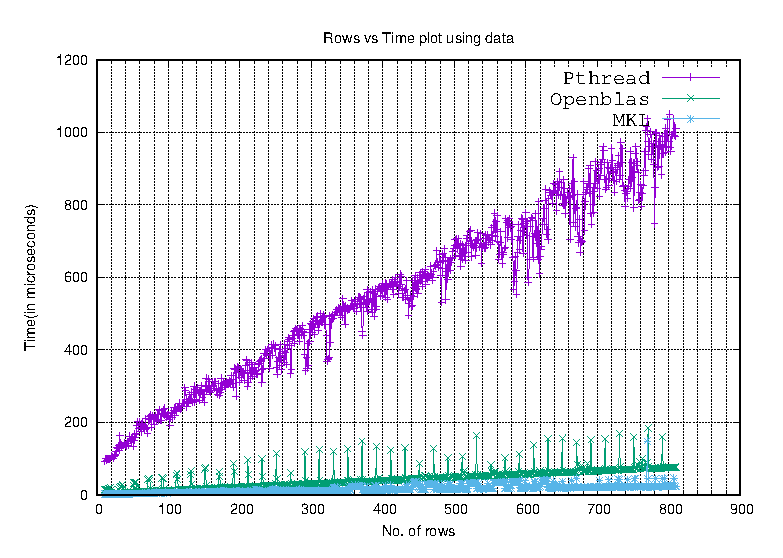
\includegraphics{All_comparision_without_error_bars.eps}
    \caption{Comparing Pthreads, openBlas and MKL}
    \label{fig:all}
\end{figure}

\subsection{Performance Comparison}
On running the libraries with suitable arguments, all of which can be found in this table, we find that MKL and OpenBlas do extremely well in comparison to our Pthreads(Figure \ref{fig:all}).


On close comparison of openBlas and MKL, we see that MKL in fact does better than openBlas, and that too with a good margin(Figure \ref{fig:openmkl}.)

\begin{figure}[hbt!]
    \centering
    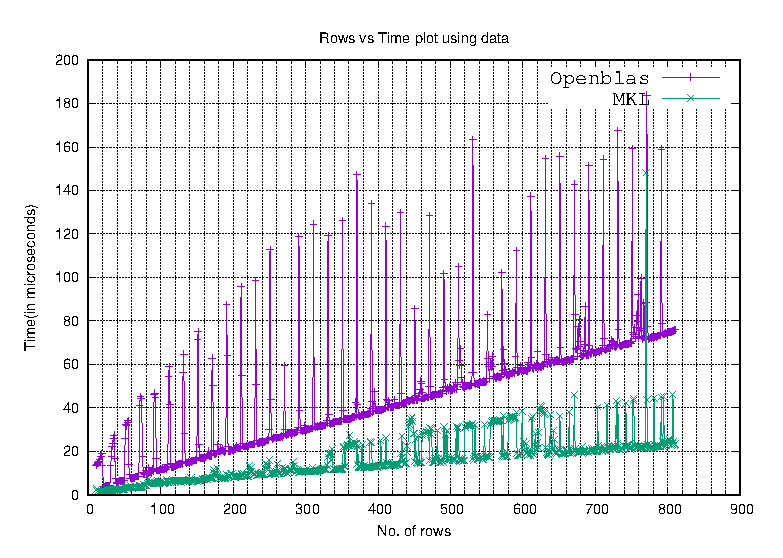
\includegraphics{openblas_vs_mkl_without_error_bars.eps}
    \caption{Comparing openBlas and MKL}
    \label{fig:openmkl}
\end{figure}
Table \ref{tab:times} contains few values which give time comparison v/s matrix size for the 3 libraries.
\begin{table}[h!]
\centering
\begin{tabular}{|l|l|l|l|}
\hline
 & \multicolumn{3}{l|}{Time (in microseconds)} \\ \hline
\begin{tabular}[c]{@{}l@{}}Matrix \\ Size\end{tabular} & Pthreads & openBlas & MKL \\ \hline
100 x 50 & 219.729 & 11.578 & 5.898 \\ \hline
110 x 50 & 239.548 & 12.6369 & 6.037 \\ \hline
120 x 50 & 252.257 & 13.35 & 6.313 \\ \hline
150 x 50 & 254.686 & 16.199 & 7.034 \\ \hline
200 x 50 & 324.321 & 20.116 & 8.728 \\ \hline
300 x 50 & 469.859 & 29.596 & 10.786 \\ \hline
400 x 50 & 582.349 & 38.894 & 12.939 \\ \hline
500 x 50 & 688.748 & 47.577 & 16.65 \\ \hline
600 x 50 & 779.342 & 57.452 & 22.320 \\ \hline
\end{tabular}
\caption{Time taken for different implementations}\label{tab:times}
\end{table}


\subsection{Some observations of including the libraries}
We found Pthreads and openBlas to be extremely user-friendly in terms of their installation. On the other hand, it was quite inconvenient to actually understand which package for the Intel MKL library would suffice. Once that was done, it was seen that manually setting up the environmental variables was in fact no good, and instead for the best experience, one must make changes to the .profile to restore the changes after shut down of the machine.\newline In addition, using the MKL Link Advisor requires the user to have a good understanding of the architecture, which served as a bottleneck for us for quite some time too. In all, we would say that though, MKL surely was the fastest of the 3 but it came with its own set of demons in its difficulty to install.
There were also some fluctuations seen when using Openblas and MKL as you may see in Figure \ref{fig:openmkl}. Occasional spikes can be due to the fact that MKL and openBlas are restarted after every 20 iterations. It was mandatory to do so, else deadlocks took place hanging the whole system.

\section{LeNet Architecture}
In the third Sub-Task, we construct our version of the LeNet architecture by using 2 Convolution layers, 2 Max-Pooling Layer and 2 Fully Connected layers. 

\subsection{Details of the layers}
The first step is to convert the given MNSIT image to an array of size 28x28. Then we store the array in the .txt file. The normalised form(values from 0-1) will be stored in the text file rather than the pixel values. 
Formula to for normalization is 
\begin{equation}
NPV = 1 - \frac{1}{255} \times pixelValues
\end{equation}
where NPV is the Normalized Pixel Values Matrix.

% MNIST Input image: 28x28 pixels, Grayscale so number of channels 1

\begin{center}
\begin{table}[hbt!]
\begin{tabularx}{\linewidth}{|X|X|X|X|X|X|X|X|X}

\cline{1-8}
Layer & Input Dimensions & Input Channels &Output Channels & Kernel Size &Padding &Output Dimensions &Acti. Fun. &  \\ \cline{1-8}
Conv 1& 28 x 28 & 1 & 20 & 5 x 5 & 0 & 24 x 24 x 20 & None   \\ \cline{1-8}
Pool 1& 24 x 24 & 20 & 20 & 2 x 2 x 20 & 0 & 12 x 12 x 20 & None   \\ \cline{1-8}
Conv 2& 12 x 12 & 20 & 50 & 5 x 5 & 0 & 8 x 8 x 50 & None   \\ \cline{1-8}
Pool 2& 8 x 8 & 50 & 50 & 2 x 2 x 50 & 0 & 4 x 4 x 50 & None  \\ \cline{1-8}
Fully Conn. 1& 4 x 4 & 50 & 500 & 4 x 4 & 0 & 1 x 1 x 500 & Relu   \\ \cline{1-8}
Fully Conn. 2& 1 x 1 & 500 & 10 & 1 x 1 & 0 & 1 x 1 x 10 & Softmax   \\ \cline{1-8}
\end{tabularx}
\caption{Layer Inputs and Outputs}\label{tab:title}
\end{table}
\end{center}

\subsection{Preprocessing and Running the data}
To preprocess the data, run
\begin{verbatim}
    python3 preprocess.py <image_file_path>
\end{verbatim}
This will output inputData.txt.
Compile the code, and run it with 
\begin{verbatim}
    make lenet
    ./lenet.out inputData.txt
\end{verbatim}
This will output the probabilities of each of the image being each of the digits from '0' to '9'. In addition, also the message for which is the most likely digit will output.

\section{Automating the Process}
For the convenience of the user a bash script automate.sh has been provided. Executing it by \begin{verbatim}
    ./automate.sh
\end{verbatim}
A UI will start in the terminal. Follow its instructions to continue.

\begin{table}[hbt!]
\caption{Design structure with the functions}\label{tab:title}
\begin{tabular}{|c|c|c|c|c|c|c|c|c|c|}
\hline
Executable & Function & \multicolumn{8}{c|}{Arguments} \\ \hline
\multirow{7}{*}{./main.out} & Sigmoid & \begin{tabular}[c]{@{}c@{}}vector\\ file\end{tabular} &  &  &  &  &  &  &  \\ \cline{2-10} 
 & Softmax & \begin{tabular}[c]{@{}c@{}}vector\\ file\end{tabular} &  &  &  &  &  &  &  \\ \cline{2-10} 
 & Tanh & \begin{tabular}[c]{@{}c@{}}matrix\\ file\end{tabular} & \begin{tabular}[c]{@{}c@{}}num\\ rows\end{tabular} &  &  &  &  &  &  \\ \cline{2-10} 
 & Relu & \begin{tabular}[c]{@{}c@{}}matrix\\ file\end{tabular} & \begin{tabular}[c]{@{}c@{}}num\\ rows\end{tabular} &  &  &  &  &  &  \\ \cline{2-10} 
 & Padding & \begin{tabular}[c]{@{}c@{}}matrix \\ file\end{tabular} & \begin{tabular}[c]{@{}c@{}}num\\ rows\end{tabular} & \begin{tabular}[c]{@{}c@{}}pad\\ num\end{tabular} &  &  &  &  &  \\ \cline{2-10} 
 & Pooling & \begin{tabular}[c]{@{}c@{}}matrix\\ file\end{tabular} & \begin{tabular}[c]{@{}c@{}}num\\ rows\end{tabular} & \begin{tabular}[c]{@{}c@{}}kernel\\ size\end{tabular} & \begin{tabular}[c]{@{}c@{}}pad\\ num\end{tabular} & \begin{tabular}[c]{@{}c@{}}pool\\ type\end{tabular} &  &  &  \\ \cline{2-10} 
 & Convolution & \begin{tabular}[c]{@{}c@{}}matrix\\ file\end{tabular} & \begin{tabular}[c]{@{}c@{}}num\\ rows\end{tabular} & \begin{tabular}[c]{@{}c@{}}kernel\\ path\end{tabular} & \begin{tabular}[c]{@{}c@{}}kernel\\ rows\end{tabular} & \begin{tabular}[c]{@{}c@{}}pad\\ type\end{tabular} & \begin{tabular}[c]{@{}c@{}}stride\\ value\end{tabular} & \begin{tabular}[c]{@{}c@{}}conv\\ type\end{tabular} & \textit{\begin{tabular}[c]{@{}c@{}}{[}mat\_\\ mul\\ type{]}\end{tabular}} \\ \hline
\multicolumn{1}{|l|}{./plot\_{[}opt{]}.out} & \multicolumn{1}{l|}{} & \multicolumn{1}{l|}{\begin{tabular}[c]{@{}l@{}}rows\\ of\\ matrix\end{tabular}} & \multicolumn{1}{l|}{\begin{tabular}[c]{@{}l@{}}rows\\ of\\ kernel\end{tabular}} & \multicolumn{1}{l|}{iters} & \multicolumn{1}{l|}{} & \multicolumn{1}{l|}{} & \multicolumn{1}{l|}{} & \multicolumn{1}{l|}{} & \multicolumn{1}{l|}{} \\ \hline
\multicolumn{1}{|l|}{./lenet.out} & \multicolumn{1}{l|}{} & \multicolumn{1}{l|}{\begin{tabular}[c]{@{}l@{}}input\\ file\end{tabular}} & \multicolumn{1}{l|}{} & \multicolumn{1}{l|}{} & \multicolumn{1}{l|}{} & \multicolumn{1}{l|}{} & \multicolumn{1}{l|}{} & \multicolumn{1}{l|}{} & \multicolumn{1}{l|}{} \\ \hline
\end{tabular}
\end{table}

\textbf{Legend}:\newline
\textbf{vector/matrix/kernel file}: string File path referencing to the txt file containing vector/matrix/kernel in column major order \newline
\textbf{num rows}: integer specifying number of rows of the previous file\newline
\textbf{pad num}: integer specifying the number of padding units\newline\textbf{newline}: string specifying the type of padding either 'same' or 'valid'\newline
\textbf{stride value}: integer specifying the stride for the kernel to take\newline
\textbf{conv type}: string specifying the type of convolution to use either "Convolution" or "Matrix".\newline
\textbf{mat\_mul\_type}: optional string. Only specify if using "Matrix" as conv type. Can be either "mkl", "openblas" or "pthreads". Leaving it blank causes it to use pthreads. 

\bibliographystyle{plain}
\bibliography{bibliography.bib}
\end{document}